\documentclass{article}
\usepackage{listings}
\usepackage{mathrsfs}
\usepackage[utf8]{inputenc}
\usepackage{amssymb}
\usepackage{lipsum}
\usepackage{amsmath}
\usepackage{fancyhdr}
\usepackage{geometry}
\usepackage{scrextend}
\usepackage[english,german]{babel}
\usepackage{titling}
\setlength{\droptitle}{-3cm}
\usepackage{tikz}
\usepackage{algorithm,algpseudocode}
\usepackage[doublespacing]{setspace}
\usetikzlibrary{datavisualization}
\usetikzlibrary{datavisualization.formats.functions}
\usepackage{polynom}
\usepackage{amsmath}
\usepackage{gauss}
\usepackage{tkz-euclide}
\usepackage{minted}
\usetikzlibrary{datavisualization}
\usetikzlibrary{datavisualization.formats.functions}
\author{
Alexander Mattick Kennung: qi69dube\\
Kapitel 1
}
\usepackage{import}
\date{\today}
\geometry{a4paper, margin=2cm}
\usepackage{stackengine}
\parskip 1em
\newcommand\stackequal[2]{%
  \mathrel{\stackunder[2pt]{\stackon[4pt]{=}{$\scriptscriptstyle#1$}}{%
  $\scriptscriptstyle#2$}}
 }
\makeatletter
\renewcommand*\env@matrix[1][*\c@MaxMatrixCols c]{%
  \hskip -\arraycolsep
  \let\@ifnextchar\new@ifnextchar
  \array{#1}}
\makeatother
\lstset{
  language=haskell,
}
\lstnewenvironment{code}{\lstset{language=Haskell,basicstyle=\small}}{}
\usepackage{enumitem}
\setlist{nosep}
\usepackage{titlesec}
\usepackage{ stmaryrd }
\usepackage{verbatim}
\usepackage{tikz-qtree}
\usepackage{bussproofs}

\titlespacing*{\subsection}{0pt}{2pt}{3pt}
\titlespacing*{\section}{0pt}{0pt}{5pt}
\titlespacing*{\subsubsection}{0pt}{1pt}{2pt}
\title{Übung 7}


\begin{document}
	\maketitle
	$X,Y\sim R(a,b)$ sind st.u\\
	\[f^{X+Y}(z) = f^X * f^Y = \int^\infty_{-\infty}f(x)f^Y(z-x)dx  \]
	\[f^{X+Y}(z) = f^X * f^Y = \frac{1}{(b-a)^2}\int^\infty_{-\infty} 1_{(a,b)}(x)1_{(a,b)}(z-x) \]
	$1_{(a,b)}(z-a)\neq 0$ falls $a<z-x<b\iff a-z<-x< b-z\iff z-b<x<z-a$\\
	$z\in (2a,2b)$ (die summe von x,y)\\
	$1_{(a,b)}(x)1_{(z-b,z-a)}(x) = 1_{(a,b)\cap (z-b,z-a)}$\\
	wir haben 2 fälle: wir haben den Fall $z-a<b$, dann ist z-a die obere und a die unter Intervallgrenze.\\
	Der Fall, wenn beide Gleich sind.\\
	Der Fall, wenn $z-b>a$, dann ist z-b die unter, b die obere.\\
	1. Fall $z-b<a$ $z-a<b\iff z<a+b$\\
	für $z\in (2a,2b)$ d.h. für $2a<z<a+b$ sind die Grenzen $y\in (a,z-a)$\dots\\
	X, Y sind NICHT st.u. dann brauchen wir die Gemeinsame Dichte (wir machen eine ``pseudo'' Faltung)
	\[f^{X+Y}(z)=\int^\infty_{-\infty}f^{(X,Y)}(x, z-x)dx\]
	Diese Gleichung gilt auch IMMER (auch bei unabhängigen), man braucht aber die Gemeinsame Dichte.\\
	im Fall der stochastischen unabhängigkeit gilt
	\[=\int_{\mathbb{R}} f^X(x)f^Y(z-x)dx\]
	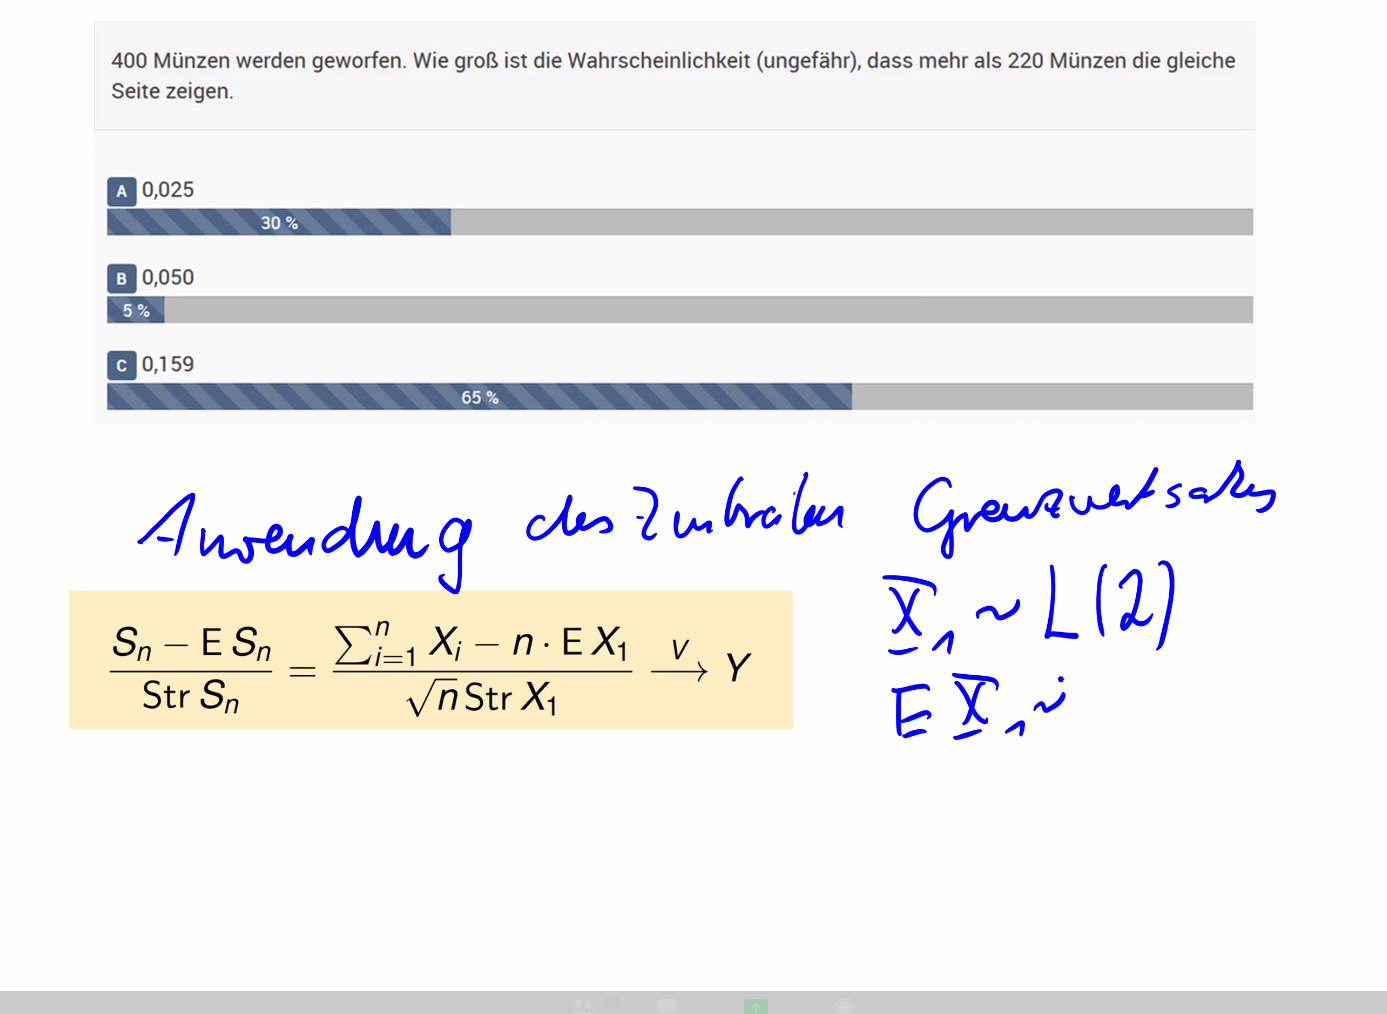
\includegraphics[height=256px]{ÜbungSchätzen.png}
	Anwendung Zentraler Grenzwertsatz. (Wir haben gleichverteilte, unabhängige Würfe)\\
	$X_1\sim L(2),\Omega_x=\{0,1\}$ oder $X_1\sim B(0.5); EX=\frac{1}{2}$\\
	$EX_1 = 0.5$\\
	$Var X_1 = 0.25\implies Str X_1 = \frac{1}{2}$\\
	\[\frac{\sum^{400}_{i=0}X_i -400\frac{1}{2}}{\sqrt{400}\frac{1}{2}} = \frac{S_{400}-200}{10}\]
	wir betrachten $S_{400} = 220$
	\[1-\Phi(\frac{220-200}{10}) = 1-\Phi(2)=1-0.97725=0.023\]
	Chebychev-Markov\\
	Verwendung im Beweis des Zentralengrenzwertsatzes.\\
	Markov-fixpunkt:\\
	wir haben eine Transitionsmatrix A mit spaltensummen 1 \\
	$x=Ax\iff (A-I)x =0$ also Eigenwerte finden.\\
	wir suchen ein $x^*\neq 0, x_i\geq 0$\\
	$x^T(A-I)^T =0$



\end{document}
